\documentclass[a4paper,12pt]{article}
\usepackage{amsmath}
\usepackage{amssymb}
\usepackage[polish]{babel}
\usepackage{polski}
\usepackage[utf8]{inputenc}
\usepackage{indentfirst}
\usepackage{geometry}
\usepackage{array}
\usepackage[pdftex]{color,graphicx}
\usepackage{subfigure}
\usepackage{afterpage}
\usepackage{setspace}
\usepackage{color}
\usepackage{wrapfig}
\usepackage{listings}
\usepackage{datetime}

\renewcommand{\onehalfspacing}{\setstretch{1.6}}

\geometry{tmargin=2.5cm,bmargin=2.5cm,lmargin=2.5cm,rmargin=2.5cm}
\setlength{\parindent}{1cm}
\setlength{\parskip}{0mm}

\newenvironment{lista}{
\begin{itemize}
  \setlength{\itemsep}{1pt}
  \setlength{\parskip}{0pt}
  \setlength{\parsep}{0pt}
}{\end{itemize}}

\newcommand{\linia}{\rule{\linewidth}{0.4mm}}

\definecolor{lbcolor}{rgb}{0.95,0.95,0.95}
\lstset{
    backgroundcolor=\color{lbcolor},
    tabsize=4,
  language=C++,
  captionpos=b,
  tabsize=3,
  frame=lines,
  numbers=left,
  numberstyle=\tiny,
  numbersep=5pt,
  breaklines=true,
  showstringspaces=false,
  basicstyle=\footnotesize,
  identifierstyle=\color{magenta},
  keywordstyle=\color[rgb]{0,0,1},
  commentstyle=\color{Darkgreen},
  stringstyle=\color{red}
  }

\begin{document}

\begin{figure}[ht]
	\centering
  
\includegraphics[width=1.0\textwidth]{p1.png}
\end{figure}
\newpage

\tableofcontents
\newpage

\section{Wprowadzenie}

W zakresie projektu zaliczeniowego zrealizowano projekt udowadniający możliwość wykorzystania oprogramowania CUDA w celu zbudowania aplikacji rozwiązującej diagramy Sudoku. CUDA to opracowana przez firmę Nvidia uniwersalna architektura procesorów wielordzeniowych, umożliwiająca wykorzystanie ich mocy obliczeniowej do rozwiązywania ogólnych problemów numerycznych w sposób wydajniejszy niż w tradycyjnych, sekwencyjnych procesorach ogólnego przeznaczenia. Powyższa platforma w doskonały sposób nadaje się do zastosowań takich jak Sudoku – gdzie możliwość wykonania setek obliczeń jednocześnie, w znaczący sposób zwiększa wydajność programu.

\section{Cel projektu}
Celem projektu jest zbudowanie aplikacji, która byłaby w stanie obliczyć diagram Sudoku o jak największym stopniu skomplikowania. Wymaga to przygotowania odpowiedniej liczy diagramów początkowych – z pustymi lukami oznaczającymi możliwość wstawienia liczby, doboru optymalnego algorytmu, który byłby w stanie dokonać obliczeń w satysfakcjonującym czasie oraz, którego budowa predysponuje do optymalnego zrównoleglenia oraz środowiska, które wspomoże odpowiednio proces implementacji i debugowania. 

\section{Środowisko implementacyjne}
Implementacja została w pełni opracowana w środowisku Microsoft Visual Studio. Jest to
zintegrowane środowisko produkcyjne (IDE) zaprojektowane przez firmę Microsoft. Jest
używane do produkcji programów komputerowych na platformę Windows. Za jego pomocą
można produkować zarówno kod natywny jak i zarządzany przez platformę .NET. Oprócz pełnego wsparcia dla platformy .NET, Visual Studio oferuje wiele narzędzi i dodatków usprawniających proces implementacji dla wielu innych technologii – również dla języka C++ i technologii CUDA.

\newpage
\section{Czym jest SUDOKU}
Sudoku jest łąmigłówką, której celem jest wypełnienie diagramu 9 x 9 w taki sposób, aby w każdym wierszu, w każdej kolumnie i w każdej z dziewięciu podtablic 3 x 3 zwanych często blokami – znalazło się po jednej unikalnej cyfrze w zakresie od 1 do 9. Zasady przypominają bardzo tzw kwadrat łaciński, wymyślony i badany przez średniowiecznych matematyków. W Sudoku w przeciwieństwie do kwadratu łacińskiego, cyfry nie mogą się powtarzać nie tylko w każdym wierszu i kolumnie ale także w mniejszych podsekcjach 3 x 3.

\begin{center}
  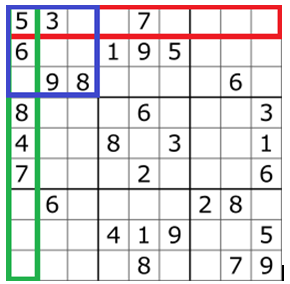
\includegraphics[scale=0.75]{p2.png}  
  \label{fig:picture2}
\end{center}
Sudoku z widocznymi miejscami do uzupełnienia i zaznaczonymi obszarami, w których wymagana jest unikalność liczby.
\section{Wybór algorytmu}
Rozważając wybór algorytmu, który byłby w stanie obliczyć diagramy o różnych stopniach trudności oraz dał się w mało kłoptliwy sposób zrównoleglić, naturalnym kandydatem była metoda Brute Force. Standardowym podejściem wykorzystania tej metody w Sudoku jest wyprodukowanie wszystkich możliwych rozwiązań a następnie sprawdzenie poprawności każdej z konfiguracji po kolei. Niestety metoda ta gwarantuje odnalezienie tylko bardzo prostych przypadków w rozsądnym czasie. W zaistniałych okolicznościach należało poszukać metody, która w podobny sposób dała by się zrównoleglić i przy okazji dawała możliwość obliczenia większego spektrum przypadków, w krótszym czasie.
Wariacją na temat techniki Brute Force jest Backtracking. Działa w podobny sposób, z wyjątkiem:

•	Poprawność wyprodukowanych wyników jest sprawdzana po każdym podjętym kroku.

•	W przypadku braku wariantów postawienia następnego kroku, istnieje możliwość powrotu do     poprzedniej decyzji i wybór innego wariantu.

W celu dodatkowego zoptymalizowania procesu wyszukiwania rozwiązania za pomocą Backtrakingu, można zastosować wcześniej przeszukiwanie wszerz (Breadth First Search).
Algorytm ten w kontekście Sudoku pozwala na zminimalizowanie wariantów potencjalnego rozwiązania poprzez wyprodukowanie x alternatywnych diagramów, które predysponują do ostatecznego uzupełniena tablicy. Odnalezione przez BFS diagramy potencjalnego rozwiązania są przekazywane do metody realizującej Backtracking, gdzie nad każdą tablicą pracuje osobny wątek. Wątki niezależnie od siebie wykonują pracę na różnych danych. Wątek, który jako pierwszy skończy pracę jest wybierany a obliczony przez niego wariant jest traktowany jako rozwiązanie. Pozostałe są odrzucane.

\section{Implementacja}

Szczegółowe etapy implementacji:

Na samym początku odbywa się sprawdzenie poprawności argumentów. Program oczekuje trzech argumentów wejściowych:

kernel.exe [liczba bloków] [liczba wątków w bloku] [ścieżka do pliku]

W następnym kroku pobierany jest plik wejściowego diagramu Sudoku. Struktura linii w pliku:

\begin{center}
  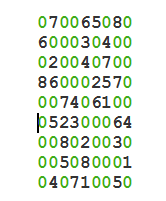
\includegraphics[scale=0.75]{p3.png}  
  \label{fig:picture}
\end{center}


Linie powinny być przedstawiane w sposób ciągły, bez pomocy żadnych separatorów. Po każdej sekwencji dziewięciu znaków umieszczany jest znak nowej linii. Symbol 0 oznacza, lukę do wypełnienia.

Struktura diagramu jest reprezentowana w programie w postaci jednowymiarowej ciągłej tablicy, mogącej przechowywac początkowy diagram jak i produkty poszczególnych algorytmów. Aby uzyskać dostęp do konkretnej tablicy, należy dokonać przesunięcia:
n * 81, dzie n to indeks konkretnej tablicy.

W następnej kolejności rejestrowane są zdarzenia CUDA a także alokowana pamięć dla wywołań kerneli.

Po przygotowaniu danych wejściowych i inicjalizacji wszystkich niezbędnych zasobów, sterowanie przejmuje metoda wykonująca algorytm BFS. Program zaczyna od pojedynczego wywołania kernela zawierającego implementację BFS. Do kernela przekazywane są dwie tablice. Źródłowa – do której wczytane została konfiguracja pierwszego diagramu oraz docelowa, do której zapisane zostaną produkty algorytmu. BFS skanuje diagram od początku, próbując odszukać następną lukę do uzupełnienia. Następnie w odnalezione miescje próbuje wstawić po kolei wszystkie możliwe wartości od 1 do 9 przy czym sprawdza czy bieżące wstawienie jest poprawne (zgodność kolumn, wierszy, podsekcji). Poprawne warianty pierwszego diagramu są zapisywane do tablicy docelowej. Jednocześnie zapamiętywana jest pozycja wszystkich pozostałych luk odnalezionego wariantu i ich liczba. Obie te informacje posłużą w późniejszych obliczeniach. 

Po pierwszym wykonaniu kernela i uzyskaniu pierwszych alternatywnych diagramów, program wykonuje cykl osiemnastu iteracji poszukiwań dalszych wariantów. W tym celu tabela źródłowa i docelowa jest zamieniana referencjami – wyniki poprzedniego przeszukiwania stanowią teraz nowe dane wejściowe dla BFS. Operacje te są powtarzane aż do skończenia cyklu iteracji. Ich produktem jest graf potencjalnych rozwiązań. Warto zauważyć, że w algorytmie BFS zastosowany został mechanizm dywergencji. Pracuje co najwyżej tyle wątków jednocześnie ile wariantów znajduje się w tablicy źródłowej. Oznacza to, że w przypadku pierwszego wywołania, pracował tylko jeden wątek.

Produkty poprzednich algorytmów są przekazywane do funkcji Backtrack.  W przeciwieństwie do poprzedniego algorytmu, który wymagał cyklu iteracji, wywołanie tego kernela, od razu przydziela każdemu wątkowi osobny diagram do rozpatrzenia. W każdym wątku program korzysta z kolekcji zapamiętanych luk. Ustawia się na kolejnej i próbuje wstawić wartości od 1 do 9. Następuje sprawdzenie kolumn, wierszy i podsekcji. W przypadku gdy diagram jest określany jako poprawny, następuje przejście do kolejnej luki. W przypadku gdy, żadna z wartości od 1 do 9 nie zagwarantowała poprawności diagramu wskaźnik jest wycofywany do miejsca ostatniej uzupełnionej luki i następuje próba wpisania alternatywnej wartości. Wygrywa wątek, który jako pierwszy odszuka w całości poprawny diagram. 

\section{Wnioski}

Algorytmy rozwiązywania Sudoku na GPU różnią się znacząco od klasycznych implementacji. Możliwość wykonania setek operacji jednocześnie oraz pewne ograniczenie technologii CUDA w stosowaniu rekursji determinują określoną manierę algorytmów. W zastosowanym podejściu ilość bloków/wątków dla optymalnego podziału zależy ściśle od rodzaju danych wejściowych. Najbardziej optymalne rozwiązanie zakłada powołanie co najwyżej takiej ilości wątków co liczba diagramów wyprodukowanych przez BFS. Przy większej liczbie wątków czas systematycznie się wydłuża z powodu kosztu ich powoływania. Zastosowane metody okazały się optymalne dla rozwiązań przypadków prostych, średniozaawansowanych i niektórch trudnych. Dla niektórych ektremalnie trudnych przypadków są niewystarczające.

\end{document}
